\section{Przypadek Testowy 3-Algorytm 2-opt: Zależność wyników od danych początkowych}
	\subsection{Cel:}
    Algorytm 2-opt bazuje na początkowej, ustalonej permutacji i na jej podstawie próbuje uzyskać lepszy wynik poprzez inwersję odpowiednich przedziałów. Celem tej części będzie sprawdzenie, jak duży wpływ ma dobór początkowej permutacji do otrzymanych wyników oraz jaki ma to wpływ na czas wykonywania algorytmu

  \subsection{Założenia:}
    Do tego badania użyto automatycznie wygenerowanych grafów typu \textbf{EUC2D}. Rozmiary grafów (oznaczane literą n) należą do zbioru $n \in \{10,15,20,...,100\}$. Do testów przygotowano 4 wartości początkowe:
    \begin{itemize}
      \item Permutację losową
      \item Permutację otrzymaną przez uruchomienie algorytmu najbliższego sąsiada na wylosowanym wierzchołku
      \item Permutację otrzymaną przez uruchomienie rozszerzonego algorytmu najbliższego sąsiada
      \item Ciąg $i \in \{1,2,...n\} $
    \end{itemize}
  \subsection{Wyniki: }

    \begin{table}[H]
    \begin{tabular}{|c | c | c | c | c |} 
     \hline
     n & Losowa & Sąsiad & Rozszerzony & Podstawowa \\ [0.5ex] 
     \hline\hline
      10 &  276 & 271 & 271 & 271 \\
      15 &  300 & 300 & 300 & 308 \\
      20 &  337 & 332 & 330 & 330 \\
      25 &  399 & 391 & 387 & 392 \\
      30 &  434 & 416 & 414 & 430 \\
      35 &  445 & 457 & 439 & 450 \\
      40 &  482 & 476 & 453 & 490 \\
      45 &  550 & 527 & 513 & 556 \\
      50 &  572 & 521 & 522 & 584 \\
      55 &  562 & 528 & 526 & 547 \\
      60 &  571 & 563 & 563 & 626 \\
      65 &  631 & 598 & 598 & 663 \\
      70 &  670 & 552 & 630 & 668 \\
      75 &  651 & 642 & 656 & 663 \\
      80 &  691 & 709 & 680 & 703 \\
      85 &  751 & 744 & 712 & 726 \\ 
      90 &  833 & 766 & 757 & 833 \\
      95 &  855 & 786 & 798 & 848 \\ 
      100 & 848 & 827 & 821 & 832 \\

     \hline
    \end{tabular}
    \caption{Funkcje celu dla zadanych grafów przy odpowiednich warunkach początkowych.}
    \end{table}


    \begin{table}[H]
    \begin{tabular}{|c | c | c | c | c |} 
     \hline
     n & Losowa & Sąsiad & Rozszerzony & Podstawowa \\ [0.5ex] 
     \hline\hline
      10 & 0.001 & 0.001 & 0.0007 & 0.004 \\
      15 & 0.015 & 0.006 & 0.002 & 0.025 \\
      20 & 0.072 & 0.025 & 0.016 & 0.073 \\
      25 & 0.142 & 0.042 & 0.031 & 0.201 \\
      30 & 0.350 & 0.036 & 0.035 & 0.363 \\
      35 & 0.720 & 0.258 & 0.058 & 0.756 \\
      40 & 1.230 & 0.411 & 0.081 & 1.314 \\
      45 & 2.106 & 0.705 & 0.234 & 2.274 \\
      50 & 3.211 & 0.473 & 0.417 & 3,319 \\
      55 & 5,068 & 1,194 & 0,994 & 5,723 \\
      60 & 7,075 & 1,531 & 1,544 & 7,512 \\
      65 & 9,536 & 1,887 & 1,883 & 11,659 \\ 
      70 & 3,957 &  1,922 & 2,811 & 15,471 \\
      75 & 21,451 &  3,926 & 1,874 & 20,245 \\
      80 & 23,508 &  6,597 & 3,218 & 27,021 \\
      85 & 30,458 &  5,715 & 4,584 & 30,862 \\
      90 & 38,122 &  5,982 & 4,108 & 41,256 \\
      95 & 4,621 &  15,187 &  6,415 & 50,381 \\
      100 & 63,692 &  12,296 &  8,039 & 64,398 \\

     \hline
    \end{tabular}
    \caption{Czas wykonania algorytmów dla zadanych grafów przy odpowiednich warunkach początkowych.}
    \end{table}

  \subsection{Wykresy: }
  \begin{figure}[H]
      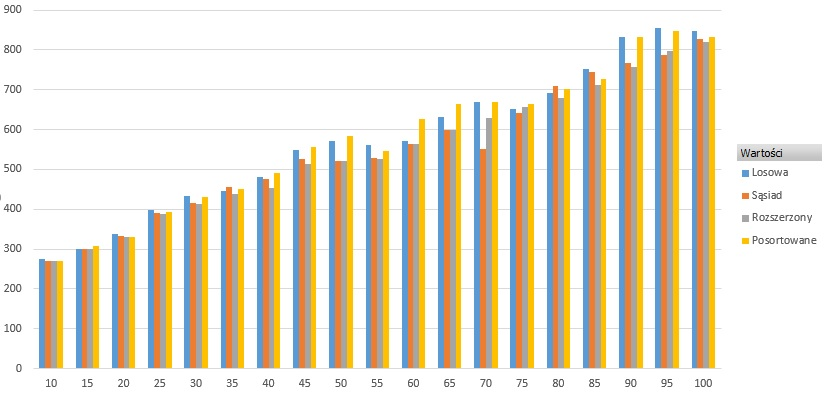
\includegraphics[scale=0.75]{droga2opt}
      \centering
      \caption{Funkcja celu dla 2-opt dla różnych startowych permutacji}
    \end{figure}
    \begin{figure}[H]
      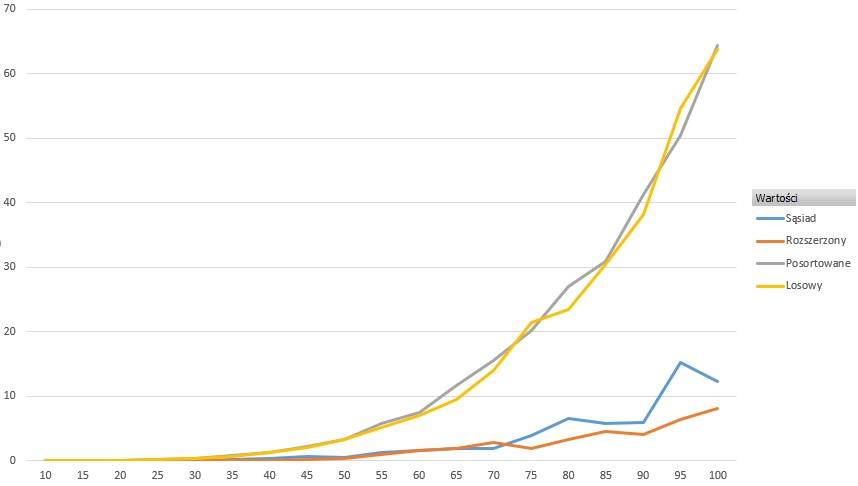
\includegraphics[scale=0.7]{czas2opt}
      \centering
      \caption{Czas dla 2-opt dla różnych startowych permutacji}
    \end{figure}
  \subsection{Wnioski: }
  Mimo podobnych wyników dla wszystkich permutacji startowych zauważamy, iz w rankingu czasowym bardzo dobrze sprawują się permutacje, które wynikają z działania algorytmu najbliższego sąsiada. Dla początkowych permutacji w formie posortowanego ciągu lub wygenerowanych losowo zauważamy złożonośc ponadliniową.
